\documentclass[11pt,a4paper]{article}
\usepackage[margin=2.4cm]{geometry}
\usepackage[T1]{fontenc}
\usepackage{lmodern}
\usepackage{amsmath,amssymb}
\usepackage{booktabs,longtable,float,graphicx,caption,array}
\usepackage[hidelinks]{hyperref}
\usepackage{xcolor}
\captionsetup{font=small,labelfont=bf}
\setlength{\parskip}{0.55em}
\setlength{\parindent}{0pt}
\renewcommand{\arraystretch}{1.12}
\newcommand{\ARIMA}[3]{\mathrm{ARIMA}(#1,#2,#3)}
\newcommand{\key}[1]{\par\medskip\noindent\fcolorbox{black!35}{black!4}{\parbox{0.955\textwidth}{#1}}\par\medskip}

\title{\textbf{Week 2: Stationarity, ARIMA Specification and Diagnostics\\for ONS UK Vacancies}}
\author{Samadrito}
\date{2 November 2026}

\begin{document}
\maketitle

\begin{abstract}
\noindent This report applies the methodology from my Week 1 review to the real ONS vacancy series (VACS02, all industries, 3-month rolling average, thousands). Using only a chronological training sample (June 2001 -- September 2024, 280 observations), with the last 24 observations held out untouched, I (1) test for stationarity and decide on the order of differencing, (2) compare 50 ARIMA$(p,1,q)$ models (plus a handful of robustness variants) using ACF/PACF plots, AIC, AICc and BIC, and (3) examine the residuals of the recommended model. \textbf{Recommendation: $\ARIMA{1}{1}{2}$ without drift, fitted to the series in levels.} Differencing once is clearly needed; the model is the best on all three information criteria; the Ljung--Box test does not reject at 6 or 12 lags, but there is modest, isolated residual autocorrelation at lags 10, 13, 16 and 24 (all below 0.16 in absolute value) and the residual variance is strongly inflated by the 2020--21 COVID-19 episode. I explain below what this means for the forecasting stage.
\end{abstract}

\tableofcontents

%--------------------------------------------------------------------
\section{Data and set-up}
%--------------------------------------------------------------------
\subsection{The series}
The workbook \texttt{vacs02oct2026.xlsx} has two sheets: ``levels'' (vacancies, thousands) and ``job openings rate''. I use the \emph{levels} sheet, column \texttt{AP2Y} (``All vacancies'', SIC 2007 sections B--S), because the Week 1 review and this brief refer to the vacancy count itself. Three facts about this series matter for everything that follows.

\begin{enumerate}
\item \textbf{It is a 3-month rolling average, published monthly.} A label such as ``Jul--Sep 2026'' is the average of July, August and September. I index each observation by the \emph{last} month of its window (so ``Jul--Sep 2026'' $\to$ September 2026). Consecutive observations therefore share two of their three underlying months. This is the point flagged under ``Points to discuss (b)'' in Week 1, and it has a concrete statistical consequence (Section~\ref{sec:acfpacf}): the differenced series has built-in autocorrelation of moving-average type.
\item \textbf{It is not seasonally adjusted, but the ONS states that it shows no seasonality} (footnote 2 of the sheet), so I do not use seasonal terms. I check this indirectly through the ACF in Section~\ref{sec:acfpacf} and the residual ACF in Section~\ref{sec:diag}: there is no spike at lags 12 or 24 that would indicate a seasonal cycle.
\item \textbf{The data run from April--June 2001 to July--September 2026}, giving 304 consecutive monthly observations (June 2001 to September 2026) with no gaps. One label in the spreadsheet contains a typo (``Nov-\,Jan 2002'', with a stray space) which a naive parser would drop, silently losing a month; my script's pattern is tolerant of this and a check asserts that the month sequence has no gaps.
\end{enumerate}

\subsection{Chronological split}
As requested, model selection uses only the earlier observations.
\begin{center}
\begin{tabular}{lll}\toprule
 & Window (month ending) & Observations\\\midrule
Training (all tests, selection, diagnostics) & June 2001 -- September 2024 & 280\\
Held out (not touched in this report) & October 2024 -- September 2026 & 24\\\bottomrule
\end{tabular}
\end{center}
The 24-month hold-out is long enough to evaluate 1-, 3- and 6-month-ahead forecasts at several origins in Week 3. One caveat: because of the rolling average, the first two hold-out values (windows ending October and November 2024) still contain August--September 2024 data that are inside the training sample. This is a property of the data, not of my split, and I flag it so that it is considered when the forecasting evaluation is designed. No test, plot-based decision or information criterion below uses any hold-out value; the hold-out is shown in grey in Figure~\ref{fig:series} only for orientation.

\begin{figure}[H]\centering
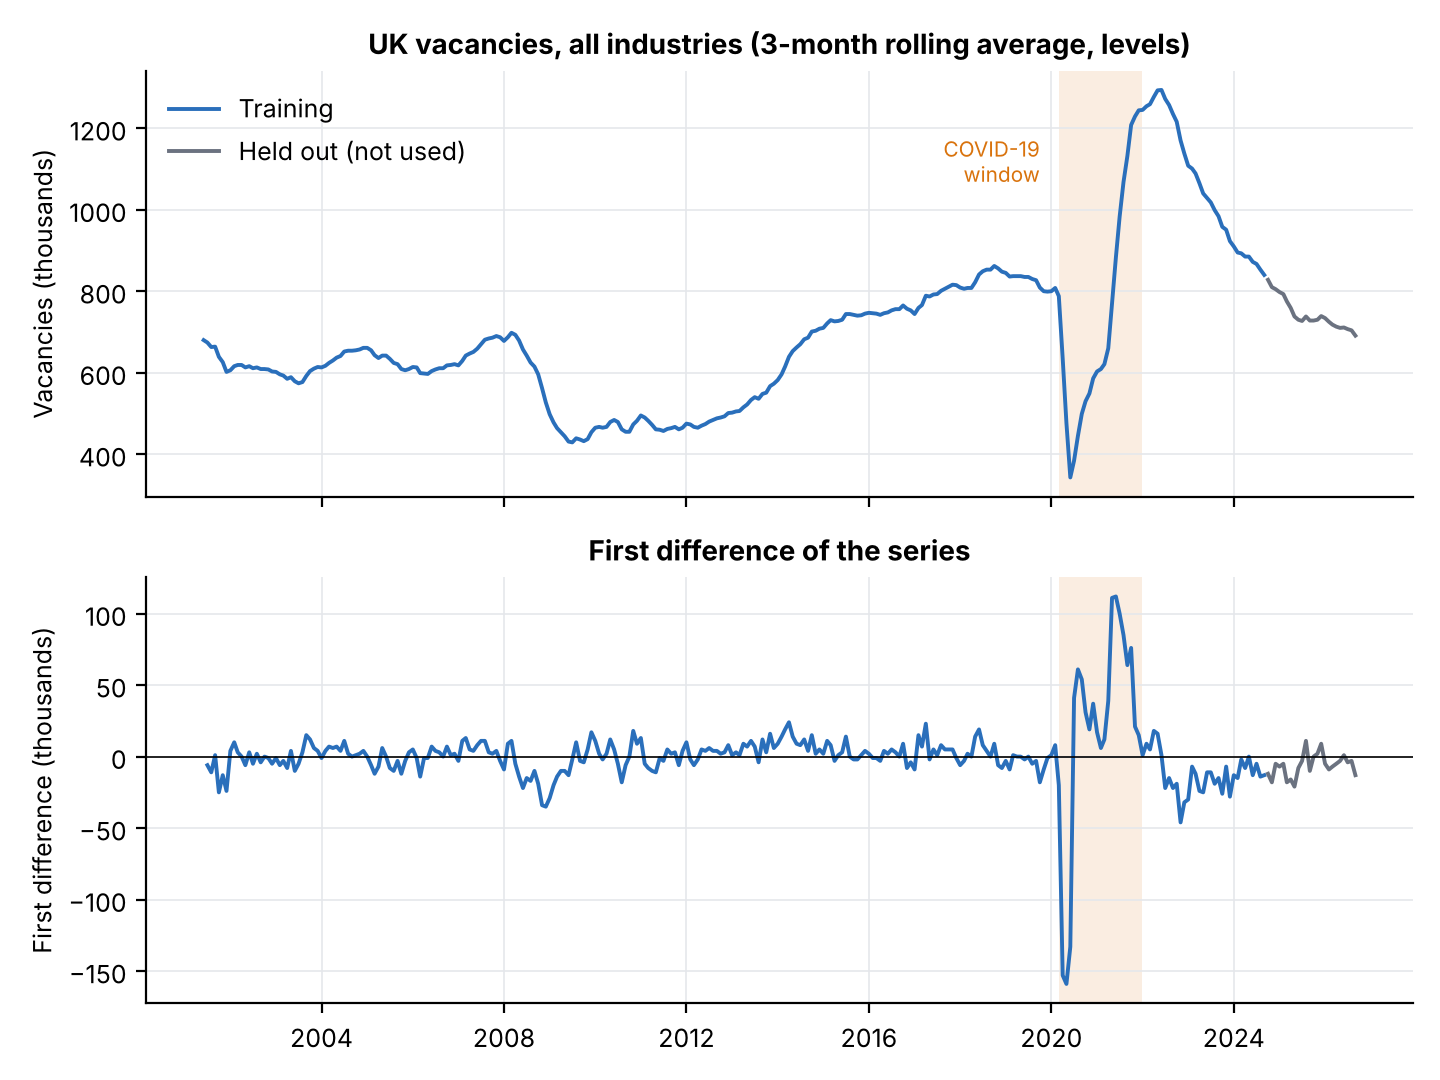
\includegraphics[width=0.92\textwidth]{figures/fig1_series.png}
\caption{Top: the vacancy series (levels, thousands), with the training sample in blue and the held-out period in grey. The shaded band marks March 2020 -- December 2021. Bottom: the first difference. The series wanders with no fixed mean (a 2009 collapse, a long recovery, the 2020 plunge, a record 1.29~million in mid-2022, then a decline), while its first difference fluctuates around zero except in the COVID window.}\label{fig:series}
\end{figure}

\subsection{Software and reproducibility}
Everything is produced by one script, \texttt{analysis.py} (Python 3.13, \texttt{statsmodels} 0.15, \texttt{scipy}, \texttt{pandas}, \texttt{matplotlib}), run as
\texttt{python3 analysis.py <vacs02.xlsx> <output dir>}. It writes every figure, every table (as CSV and as \LaTeX{}) and the numerical results quoted below. ARIMA models are fitted by exact Gaussian maximum likelihood (\texttt{statsmodels.tsa.arima.model.ARIMA}); for $d=1$ the first observation initialises the differenced process with a diffuse prior, so the first residual is a start-up artefact and is dropped from all residual diagnostics, and the likelihood of all models is computed on the same 279 differenced observations, which makes the information criteria comparable.

%--------------------------------------------------------------------
\section{Task 1: Stationarity and differencing}
%--------------------------------------------------------------------
\subsection{What is being tested and why two tests}
A series is (weakly) stationary if its mean, variance and autocovariances do not depend on time. ARIMA's AR and MA terms estimate fixed patterns, so they need a stationary series to work with; differencing ($d>0$) is the remedy for a unit root.

\textbf{Augmented Dickey--Fuller (ADF).} Regress $\Delta y_t$ on a constant (and optionally a linear trend), on $y_{t-1}$ and on $k$ lagged differences:
\[
\Delta y_t = \alpha + \beta t + \gamma\, y_{t-1} + \sum_{i=1}^{k}\delta_i \Delta y_{t-i} + e_t .
\]
The null hypothesis is a \emph{unit root} ($\gamma=0$); a large negative $t$-statistic on $\gamma$ rejects it, i.e.\ supports stationarity. The lagged differences absorb autocorrelation in $e_t$. I report two choices of $k$ (chosen by AIC and by BIC), since the answer can be sensitive to it, and two deterministic specifications (constant only; constant and trend).

\textbf{KPSS.} KPSS reverses the roles: its null is that the series is \emph{stationary} (around a level, or around a trend), and a large statistic rejects it in favour of a unit root. The two tests have opposite nulls, so using both gives a confirmatory check. The useful reading is:
\begin{center}\small
\begin{tabular}{lll}\toprule
ADF & KPSS & Conclusion\\\midrule
rejects unit root & does not reject stationarity & stationary\\
does not reject & rejects & unit root, difference the series\\
both reject / neither rejects & & inconclusive (e.g.\ outliers, low power)\\\bottomrule
\end{tabular}
\end{center}
As the Week 1 review put it, the outcome is a guide, not a verdict, so I also look at plots and at the ACF.

\subsection{Results on the original and differenced series}
Table~\ref{tab:stat_main} gives the tests on the training sample.
\begin{table}[H]\centering\small
\caption{Unit-root and stationarity tests on the training sample (June 2001 -- September 2024).}\label{tab:stat_main}
\resizebox{\textwidth}{!}{\begin{tabular}{lcccccc}\toprule
 & \multicolumn{4}{c}{ADF (H$_0$: unit root)} & \multicolumn{2}{c}{KPSS (H$_0$: stationary)}\\
\cmidrule(lr){2-5}\cmidrule(lr){6-7}
Series & const, AIC & const, BIC & c+trend, AIC & c+trend, BIC & level & trend\\\midrule
Level & $-$1.37 (0.595) & $-$2.89 (0.046) & $-$2.38 (0.388) & $-$3.85 (0.014) & 1.26 ($\leq$0.01) & 0.31 ($\leq$0.01)\\
1st difference & $-$5.67 ($<$0.001) & $-$4.00 (0.001) & $-$5.67 ($<$0.001) & $-$3.98 (0.009) & 0.06 ($\geq$0.10) & 0.04 ($\geq$0.10)\\
2nd difference & $-$5.43 ($<$0.001) & $-$11.11 ($<$0.001) & $-$5.43 ($<$0.001) & $-$11.10 ($<$0.001) & 0.11 ($\geq$0.10) & 0.10 ($\geq$0.10)\\
log~Level & $-$2.46 (0.126) & $-$2.26 (0.184) & $-$3.46 (0.044) & $-$2.93 (0.152) & 1.18 ($\leq$0.01) & 0.31 ($\leq$0.01)\\
log~1st difference & $-$4.65 ($<$0.001) & $-$6.21 ($<$0.001) & $-$4.64 ($<$0.001) & $-$6.19 ($<$0.001) & 0.07 ($\geq$0.10) & 0.04 ($\geq$0.10)\\
\bottomrule
\end{tabular}}
\par\smallskip\footnotesize Each cell: test statistic (p-value). ``AIC''/``BIC'' = rule used to choose the number of augmenting lags. ADF 5\% critical values are about $-2.87$ (constant) and $-3.42$ (constant + trend). KPSS p-values are interpolated and truncated to [0.01, 0.10].
\end{table}

\textbf{Original (level) series.}
\begin{itemize}
\item The ADF test with AIC-chosen lags (15 lags) does \emph{not} reject a unit root (statistic $-1.37$, $p=0.595$; with a trend $-2.38$, $p=0.388$).
\item With BIC-chosen lags (7 lags) the ADF test rejects narrowly ($p=0.046$ with a constant, $p=0.014$ with a trend).
\item KPSS rejects stationarity decisively under both nulls (statistics $1.26$ and $0.31$ against 5\% critical values $0.463$ and $0.146$; $p\le 0.01$).
\item The lag-1 autocorrelation of the level is $0.993$, and the ACF decays only very slowly (Figure~\ref{fig:acf}, top left). An AR(1) with constant fitted to the levels gives $\hat\phi=0.991$ (s.e.\ $0.007$), indistinguishable from the unit-root boundary.
\end{itemize}
The two ADF variants disagree, so the ADF alone would be borderline. The evidence nevertheless points one way. KPSS rejects strongly, the slowly decaying ACF is the textbook symptom of a unit root, and the ADF rejection under BIC lags is fragile: it appears or disappears with the lag rule. A plausible reason is the 2020--21 V-shaped collapse and rebound, which looks like fast mean reversion to the ADF regression and can inflate its power to reject. The pre-COVID sub-sample test below supports this reading.

\textbf{First difference.} Every ADF variant rejects a unit root ($p\le 0.009$; statistics between $-3.98$ and $-5.67$), and KPSS does not reject stationarity (statistics $0.057$ and $0.043$, both below the 10\% critical values). Both tests agree, so the first-differenced series is stationary in the sense that matters for ARIMA modelling.

\textbf{Second difference.} Also stationary on every test, as expected: a stationary series stays stationary when differenced again. That does not mean $d=2$ is needed. Needing a second difference would require evidence that the \emph{first difference} still has a unit root, and the tests above reject exactly that.

\begin{figure}[H]\centering
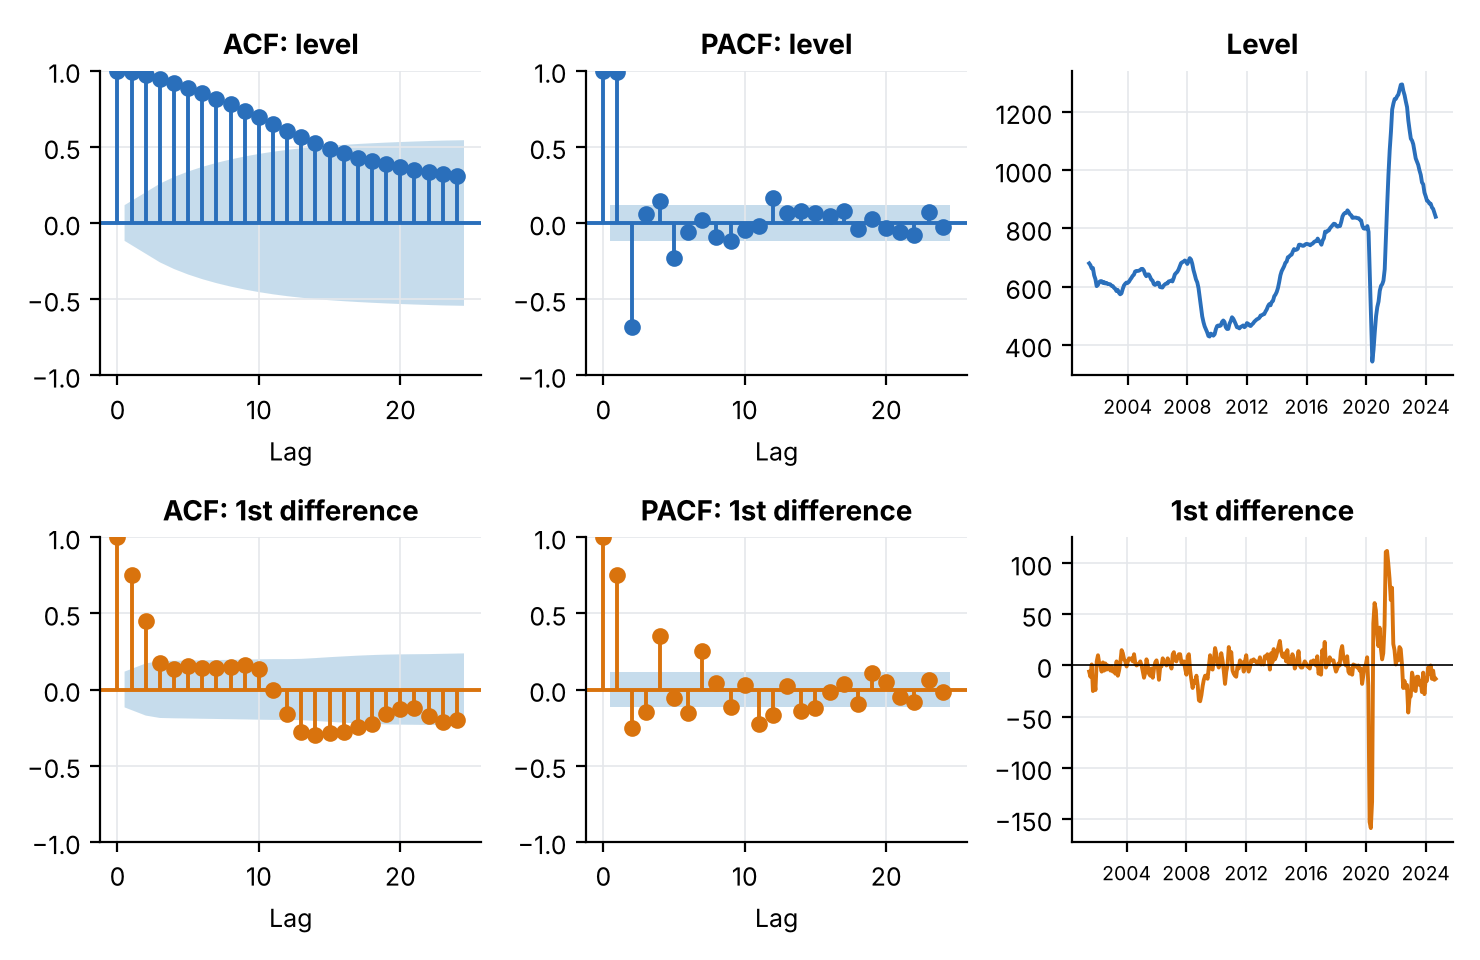
\includegraphics[width=0.97\textwidth]{figures/fig2_acf_pacf.png}
\caption{ACF and PACF of the training series in levels (top) and first differences (bottom). Shaded bands are approximate 95\% intervals. The level ACF decays slowly (non-stationary); the differenced ACF drops quickly, with the PACF showing a large first partial autocorrelation.}\label{fig:acf}
\end{figure}

\subsection{Is first differencing enough, or too much?}
A common check for over-differencing is whether the differenced series has a large negative lag-1 autocorrelation (near $-0.5$) or a larger variance than before. Here:
\begin{center}\small
\begin{tabular}{lrrr}\toprule
 & Level ($d=0$) & First difference & Second difference\\\midrule
Standard deviation & 198.8 & 24.2 & 17.1\\
Lag-1 autocorrelation & 0.993 & 0.750 & $+0.098$\\\bottomrule
\end{tabular}
\end{center}
The second difference has a \emph{positive} lag-1 autocorrelation, so there is no over-differencing signature. The standard deviation does fall slightly from $d=1$ to $d=2$, which the ``choose the $d$ with minimum variance'' rule of thumb would read as favouring $d=2$. I do not follow that rule here, because the first difference is itself strongly autocorrelated (lag-1 correlation $0.75$, a consequence of the 3-month averaging), so differencing it again mechanically removes some variance without that being a sign of a unit root. The formal tests (ADF rejects, KPSS does not reject, for $\Delta y_t$) are the better guide and they say $d=1$.

The first differences also look stable over time apart from the COVID window (Figure~\ref{fig:series}, bottom, and Figure~\ref{fig:rolling}).
\begin{figure}[H]\centering
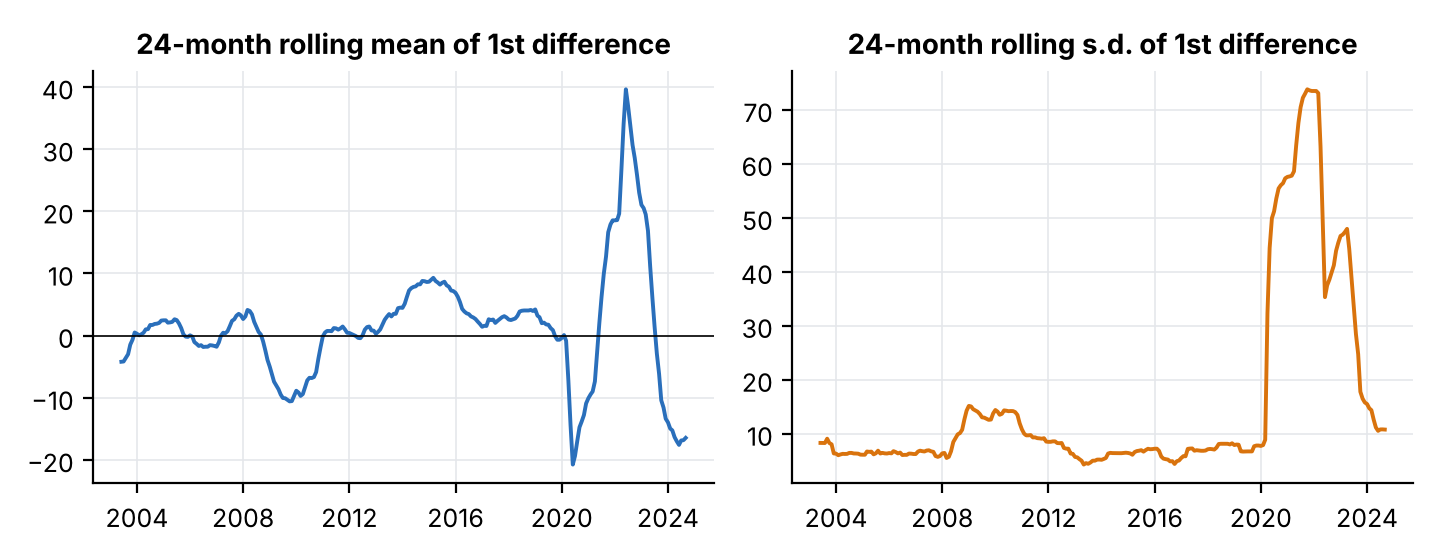
\includegraphics[width=0.9\textwidth]{figures/fig3_rolling.png}
\caption{24-month rolling mean and standard deviation of the first difference. The mean stays near zero apart from the COVID swing; the spread is stable except for that episode.}\label{fig:rolling}
\end{figure}

\subsection{Robustness: log scale and sub-samples}
\begin{table}[H]\centering\small
\caption{Sub-sample tests. The post-COVID sample has only 33 observations, so these tests have little power.}\label{tab:stat_sub}
\resizebox{\textwidth}{!}{\begin{tabular}{lcccccc}\toprule
 & \multicolumn{4}{c}{ADF (H$_0$: unit root)} & \multicolumn{2}{c}{KPSS (H$_0$: stationary)}\\
\cmidrule(lr){2-5}\cmidrule(lr){6-7}
Series & const, AIC & const, BIC & c+trend, AIC & c+trend, BIC & level & trend\\\midrule
Pre-COVID level (to Dec 2019) & $-$1.40 (0.583) & $-$1.37 (0.598) & $-$1.89 (0.660) & $-$1.73 (0.738) & 0.82 ($\leq$0.01) & 0.45 ($\leq$0.01)\\
Pre-COVID 1st diff & $-$3.50 (0.008) & $-$4.19 ($<$0.001) & $-$3.55 (0.035) & $-$4.14 (0.006) & 0.30 ($\geq$0.10) & 0.09 ($\geq$0.10)\\
Post-COVID level (from Jan 2022) & $-$1.05 (0.734) & 0.46 (0.984) & $-$1.99 (0.606) & $-$2.40 (0.382) & 0.74 (0.010) & 0.11 ($\geq$0.10)\\
Post-COVID 1st diff & $-$3.28 (0.016) & $-$3.03 (0.032) & $-$2.27 (0.452) & $-$3.13 (0.100) & 0.17 ($\geq$0.10) & 0.15 (0.043)\\
\bottomrule
\end{tabular}}
\par\smallskip\footnotesize Each cell: test statistic (p-value). ``AIC''/``BIC'' = rule used to choose the number of augmenting lags. ADF 5\% critical values are about $-2.87$ (constant) and $-3.42$ (constant + trend). KPSS p-values are interpolated and truncated to [0.01, 0.10].
\end{table}
\begin{itemize}
\item \textbf{Log scale} (Table~\ref{tab:stat_main}, bottom rows): the conclusion is the same, and slightly cleaner. The ADF fails to reject a unit root in the log level under three of four specifications ($p=0.126,\,0.184,\,0.152$; the exception is $p=0.044$ with trend and AIC lags), KPSS rejects, and the log first difference is stationary on every test.
\item \textbf{Pre-COVID sample} (June 2001 -- December 2019, 223 observations): free of the 2020--21 shock, the level series is clearly non-stationary (ADF $p=0.58$ and $0.60$ with a constant, $p=0.66$ and $0.74$ with a trend; KPSS rejects), and its first difference is stationary (ADF $p\le 0.035$; KPSS does not reject). This supports the interpretation above: the unit-root conclusion is not an artefact of COVID; it is the borderline ADF rejection on the full sample that is.
\item \textbf{Post-COVID sample} (from January 2022, 33 observations): too short for the tests to have power, and results are mixed (e.g.\ KPSS with trend rejects for the differenced series, $p=0.043$). I report it for completeness but give it no weight.
\end{itemize}

\key{\textbf{Conclusion for Task 1.} Use $d=1$. The level series is non-stationary (KPSS rejects, slowly decaying ACF, AR(1) coefficient of $0.991$, pre-COVID ADF cannot reject), the first difference is stationary on all ADF and KPSS variants, and a second difference is unnecessary (no over-differencing signature; stationarity of $\Delta y_t$ is not rejected). The conclusion is the same on the log scale and without the COVID period.}

%--------------------------------------------------------------------
\section{Task 2: Comparing ARIMA specifications}
%--------------------------------------------------------------------
\subsection{Reading the ACF and PACF of the differenced series}\label{sec:acfpacf}
With $d=1$, Figure~\ref{fig:acf} (bottom) gives the starting points for $p$ and $q$ (band $\pm 0.117$ for 279 observations):
\begin{center}\small
\begin{tabular}{lrrrrrr}\toprule
Lag & 1 & 2 & 3 & 4 & 5 & 6\\\midrule
ACF of $\Delta y_t$ & 0.750 & 0.451 & 0.173 & 0.136 & 0.153 & 0.142\\
PACF of $\Delta y_t$ & 0.750 & $-0.255$ & $-0.146$ & 0.354 & $-0.053$ & $-0.155$\\\bottomrule
\end{tabular}
\end{center}
The ACF falls off sharply after lag 2 (from 0.45 to 0.17), which suggests an MA component of order about 2. The PACF has several significant spikes (lags 1, 2, 3, 4, \dots), so a pure AR model would need many terms. These are only suggestions, but there is a structural reason to take $q=2$ seriously: if the underlying \emph{monthly} series had uncorrelated changes $\varepsilon_t$, its 3-month moving average would have $\Delta y_t=(\varepsilon_t+\varepsilon_{t-1}+\varepsilon_{t-2})/3$, which is exactly an MA(2) process (theoretical autocorrelations $2/3$ and $1/3$ at lags 1 and 2, zero afterwards). The observed values ($0.75$, $0.45$) are larger, consistent with that MA(2) structure \emph{plus} genuine persistence in monthly changes, which an AR term can capture. This points to a small ARMA$(p,2)$ model for $\Delta y_t$.

\subsection{Candidate set and criteria}
I fitted $\ARIMA{p}{1}{q}$ for every $0\le p,q\le 4$, each with and without a drift term (a constant in the differenced series, i.e.\ a linear trend in the level): 50 models, all on the same 280 observations and same $d$, so that their information criteria are comparable. The criteria are
\[
\mathrm{AIC}=-2\ell+2k,\qquad \mathrm{AICc}=\mathrm{AIC}+\frac{2k(k+1)}{n-k-1},\qquad \mathrm{BIC}=-2\ell+k\ln n,
\]
where $\ell$ is the maximised log-likelihood, $k$ the number of estimated parameters (including the innovation variance) and $n=279$ the number of differenced observations. Smaller is better. BIC penalises extra parameters more heavily than AIC and is therefore the more conservative guide, which was the reasoning in Week 1 for short samples; AICc corrects AIC for small $n/k$. As a rule of thumb, a difference of 0--2 between two models means no meaningful preference, 4--7 is clear evidence, and more than 10 is strong. Information criteria measure fit net of complexity; they do not say whether a model's residuals are clean, so I use the Ljung--Box test as a second criterion (the adequacy check requested in Task~3), with its degrees of freedom reduced by $p+q$.

I do not compare models with different $d$ by information criteria (not valid, because the differenced data differ), which is why $d$ was settled first by the tests in Task~1.

\subsection{Comparison table}
Table~\ref{tab:candidates} compares a short list: the naive random walk $(0,1,0)$ as the floor, the standard low-order models, and the leading models from the full grid. The complete 50-model grid is in \texttt{tables/arima\_grid\_full.csv} and the top 15 by BIC are in Appendix~\ref{app:top15}.
\begin{table}[H]\centering\small
\caption{Candidate ARIMA$(p,1,q)$ specifications on the training sample ($n=280$, 279 differenced observations). $\Delta$ = difference from the best value in the full 50-model grid; bold Ljung--Box p-values are below 0.05.}\label{tab:candidates}
\resizebox{\textwidth}{!}{\begin{tabular}{lcrrrrrrrrr}\toprule
Model & $k$ & AIC & AICc & BIC & $\Delta$AIC & $\Delta$BIC & $\hat\sigma$ & LB(6) & LB(12) & LB(24)\\\midrule
ARIMA(0,1,0) & 1 & 2570.0 & 2570.0 & 2573.6 & 322.6 & 311.7 & 24.12 & \textbf{0.000} & \textbf{0.000} & \textbf{0.000}\\
ARIMA(0,1,1) & 2 & 2419.1 & 2419.1 & 2426.4 & 171.7 & 164.5 & 18.33 & \textbf{0.000} & \textbf{0.000} & \textbf{0.000}\\
ARIMA(1,1,1) & 3 & 2332.2 & 2332.3 & 2343.1 & 84.9 & 81.2 & 15.62 & \textbf{0.000} & \textbf{0.000} & \textbf{0.000}\\
ARIMA(0,1,2) & 3 & 2254.8 & 2254.9 & 2265.7 & 7.4 & 3.8 & 13.55 & \textbf{0.005} & \textbf{0.008} & \textbf{0.000}\\
ARIMA(1,1,2)$^\star$ & 4 & 2247.4 & 2247.5 & 2261.9 & 0.0 & 0.0 & 13.32 & 0.474 & 0.199 & \textbf{0.006}\\
ARIMA(2,1,2) & 5 & 2249.2 & 2249.5 & 2267.4 & 1.9 & 5.5 & 13.32 & 0.282 & 0.151 & \textbf{0.005}\\
ARIMA(0,1,3) & 4 & 2248.0 & 2248.2 & 2262.6 & 0.7 & 0.7 & 13.33 & 0.367 & 0.151 & \textbf{0.003}\\
ARIMA(1,1,3) & 5 & 2249.0 & 2249.2 & 2267.2 & 1.7 & 5.3 & 13.31 & 0.223 & 0.135 & \textbf{0.007}\\
ARIMA(1,1,4) & 6 & 2249.6 & 2249.9 & 2271.4 & 2.3 & 9.5 & 13.28 & 0.264 & 0.148 & \textbf{0.009}\\
ARIMA(1,1,2)$+$drift & 5 & 2249.3 & 2249.6 & 2267.5 & 2.0 & 5.6 & 13.32 & 0.473 & 0.199 & \textbf{0.006}\\
\bottomrule
\end{tabular}}
\par\smallskip\footnotesize $k$ counts all estimated parameters including the innovation variance. LB($m$): Ljung--Box p-value using $m$ lags and $m-p-q$ degrees of freedom. $^\star$ recommended. ARIMA(0,1,0) has no estimated mean, so $k=1$ (the variance) and LB uses no degree-of-freedom correction.
\end{table}

\begin{figure}[H]\centering
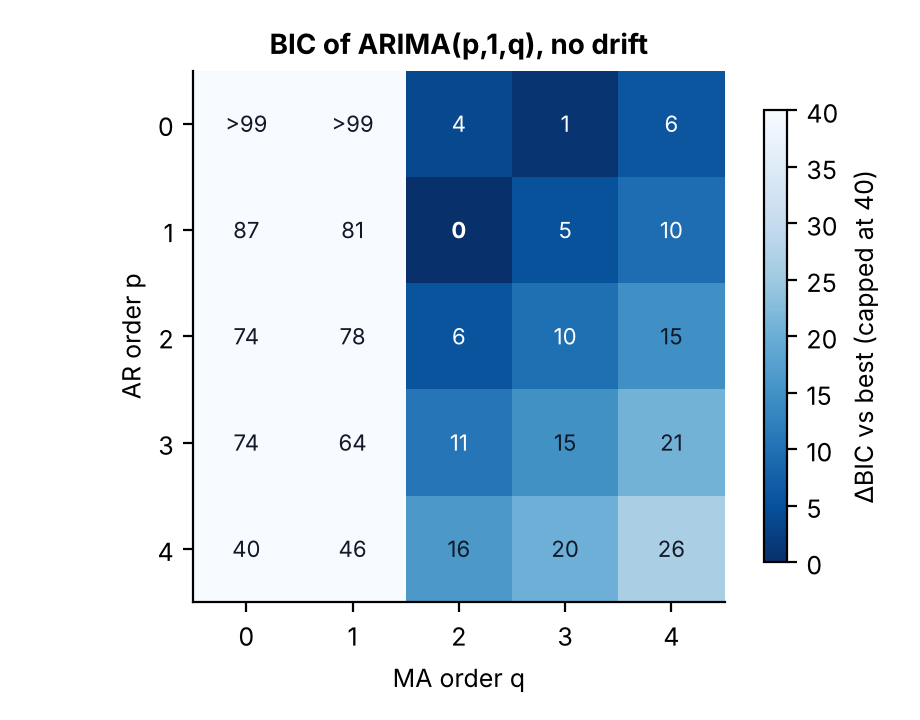
\includegraphics[width=0.6\textwidth]{figures/fig4_bic_heatmap.png}
\caption{$\Delta$BIC relative to the best model for each $(p,q)$ with $d=1$ and no drift. Models with $q\le 1$ are far worse (the MA(2) structure is essential); beyond $q=2$ and $p=1$, extra terms do not help.}\label{fig:heat}
\end{figure}

\textbf{What the evidence says.}
\begin{itemize}
\item \textbf{$q\ge 2$ is essential.} Going from $(0,1,1)$ to $(0,1,2)$ lowers BIC by about 161 points; $q\le 1$ models are rejected by every criterion (Figure~\ref{fig:heat}) and have Ljung--Box p-values of essentially zero. This matches the ACF reading and the moving-average structure of the data.
\item \textbf{$\ARIMA{1}{1}{2}$ is best on all three criteria} (AIC 2247.4, AICc 2247.5, BIC 2261.9). Adding an AR(1) term to the $(0,1,2)$ model improves BIC by 3.8 and AIC by 7.4 and fixes the short-lag residual autocorrelation (LB(6) rises from 0.005 to 0.47, LB(12) from 0.008 to 0.20).
\item \textbf{$\ARIMA{0}{1}{3}$ is a close competitor} (BIC 0.7 higher, AIC 0.7 higher). A $\Delta$BIC of 0.7 is no real distinction, and the model has the same number of parameters. I prefer $(1,1,2)$ because it is ranked first by all criteria and because the AR(1) term has a clear interpretation (persistence of monthly changes) on top of the averaging-induced MA(2).
\item \textbf{More complex models do not earn their keep.} $(2,1,2)$, $(1,1,3)$ and $(1,1,4)$ have BIC 5.3--9.5 higher (clear evidence against) and AIC 1.7--2.3 higher as well, so the extra terms do not improve fit enough to pay for themselves.
\item \textbf{Drift is not needed.} Adding a drift to $(1,1,2)$ increases AIC by 2.0 and BIC by 5.6; the estimated drift is 0.42 thousand per month with $p=0.91$. This is expected for a series that rises and falls over time.
\item \textbf{The naive $(0,1,0)$ model} is more than 300 BIC points worse than the best model, confirming that there is substantial short-run dynamics to exploit.
\end{itemize}

\subsection{Is the choice robust?}
Table~\ref{tab:robust} repeats the $0\le p,q\le 4$ search under alternative treatments of the data.
\begin{table}[H]\centering\small
\caption{Does the choice of specification survive alternative treatments? Each row repeats the 25-model ARIMA$(p,1,q)$ grid ($0\le p,q\le4$, no drift).}\label{tab:robust}
\resizebox{\textwidth}{!}{\begin{tabular}{lccrrr}\toprule Treatment & Best BIC & Best AIC & $\Delta$BIC of (1,1,2) & LB(12) & LB(24)\\\midrule
Training sample, levels (baseline) & (1,1,2) & (1,1,2) & 0.0 & 0.199 & \textbf{0.006}\\
Training sample, log levels & (0,1,2) & (0,1,2) & 5.4 & 0.220 & 0.348\\
Pre-COVID only (Jun 2001--Dec 2019) & (1,1,4) & (1,1,4) & 6.7 & 0.432 & 0.182\\
Training sample + 4 outlier dummies & (0,1,3) & (0,1,3) & 1.6 & 0.280 & \textbf{0.008}\\
\bottomrule\end{tabular}}
\par\smallskip\footnotesize LB columns refer to the best-BIC model of that row. Dummies are single-month additive outliers at Apr 2020, Jul 2020, May 2021, Aug 2021 (months with $|z|>3$ in the baseline residuals; chosen after inspecting residuals, so this is a sensitivity check, not an independent test).
\end{table}
\begin{itemize}
\item \textbf{Log scale.} The best model is $(0,1,2)$, with $(1,1,2)$ 5.4 BIC points behind. Raw information criteria from log and level fits are \emph{not} comparable, because the likelihoods refer to different variables. Table~\ref{tab:lvslog} converts the log-scale criteria to the scale of the original data (adding $2\sum_t\ln y_t$, the Jacobian of the transformation). On that fair comparison, the level model is better by 168 BIC points: modelling the log series fits the data markedly worse, even though its Ljung--Box test at lag 24 is cleaner (0.35). The log residuals also show very strong volatility clustering around 2020 (ARCH-LM $p<0.001$), because the log transformation magnifies the proportional size of the 2020 collapse. I therefore stay on the level scale.
\item \textbf{Pre-COVID only.} The best model becomes $(1,1,4)$ and passes the lag-12 and lag-24 Ljung--Box tests; $(1,1,2)$ is 6.7 BIC points behind. The qualitative picture, $q\ge2$ plus a single AR term, is the same, but with the COVID shock out of the sample a longer MA structure is favoured. This is useful information about the stability of the specification: it is possible that the COVID months push the full-sample fit towards the more parsimonious $(1,1,2)$.
\item \textbf{Outlier dummies.} Adding single-month additive-outlier dummies for the four months with $|z|>3$ (Section~\ref{sec:diag}) makes $(0,1,3)$ the best model, with $(1,1,2)$ only 1.6 BIC points behind, a statistical tie. The $(1,1,2)$ coefficients barely move ($\hat\phi_1=0.31$ vs.\ $0.22$, $\hat\theta_1=0.90$ vs.\ $0.83$, $\hat\theta_2=0.77$ vs.\ $0.81$). Because these months were identified from the baseline residuals, this is a sensitivity check rather than an independent test.
\end{itemize}
\begin{table}[H]\centering\small
\caption{Levels versus log levels. Log-scale AIC/BIC have been converted to the scale of the original data by adding $2\sum_t \log y_t$, so the four rows are directly comparable.}\label{tab:lvslog}
\begin{tabular}{llrrrrrr}\toprule Scale & Model & Adj.\ AIC & Adj.\ BIC & $\Delta$BIC & LB(12) & LB(24) & ARCH-LM\\\midrule
Levels & ARIMA(1,1,2) & 2247.4 & 2261.9 & 0.0 & 0.199 & \textbf{0.006} & 0.135\\
Levels & ARIMA(0,1,2) & 2254.8 & 2265.7 & 3.8 & \textbf{0.008} & \textbf{0.000} & 0.333\\
Log levels & ARIMA(0,1,2) & 2419.3 & 2430.2 & 168.3 & 0.220 & 0.348 & \textbf{0.000}\\
Log levels & ARIMA(1,1,2) & 2421.1 & 2435.6 & 173.7 & 0.164 & 0.335 & \textbf{0.000}\\
\bottomrule\end{tabular}
\end{table}

\subsection{Recommended specification and its estimates}
\key{\textbf{Recommendation: $\ARIMA{1}{1}{2}$, no drift, on the series in levels.}\\[2pt]
$(1-\phi_1 B)(1-B)\,y_t=(1+\theta_1 B+\theta_2 B^2)\,\varepsilon_t,\qquad \varepsilon_t\sim(0,\sigma^2)$.}
\begin{table}[H]\centering\small
\caption{Maximum-likelihood estimates, ARIMA(1,1,2), no drift, training sample.}\label{tab:params}
\begin{tabular}{lrrrrr}\toprule Parameter & Estimate & Std.\ error & $z$ & p-value & 95\% CI\\\midrule
$\phi_1$ (AR 1) & 0.218 & 0.076 & 2.86 & 0.004 & [0.068, 0.367]\\
$\theta_1$ (MA 1) & 0.831 & 0.045 & 18.38 & $<$0.001 & [0.742, 0.919]\\
$\theta_2$ (MA 2) & 0.812 & 0.021 & 37.96 & $<$0.001 & [0.770, 0.854]\\
$\sigma^2$ & 177.386 & 5.323 & 33.33 & $<$0.001 & [166.954, 187.818]\\
\bottomrule\end{tabular}
\end{table}
All three coefficients are significant. The AR coefficient $\hat\phi_1=0.22$ is modest: a month's change carries over about a fifth into the next. The MA coefficients ($0.83$ and $0.81$) are close to $(1,1)$, which is the pattern a 3-month moving average of an underlying series with uncorrelated changes would produce ($1+B+B^2$). Both roots of the MA polynomial have modulus $1.11$: the model is invertible, but close to the boundary. This is a sign that the ``averaging'' structure is being picked up almost exactly, and it means that parameter estimates and standard errors should be treated with some caution (near-boundary MA models have non-standard sampling behaviour).

Figure~\ref{fig:fitted} shows the one-step fitted monthly change against the actual change in the training sample since 2012.
\begin{figure}[H]\centering
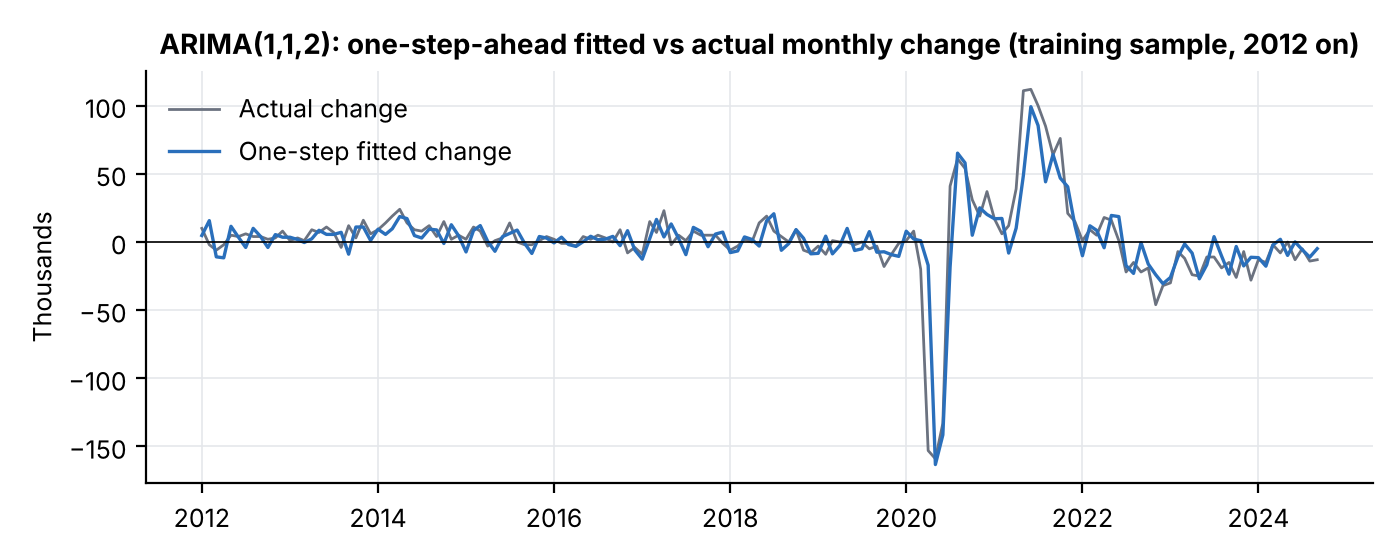
\includegraphics[width=0.95\textwidth]{figures/fig7_fitted.png}
\caption{One-step-ahead in-sample fitted vs.\ actual monthly change in the vacancy series (training sample, 2012 onwards, which includes the COVID shock).}\label{fig:fitted}
\end{figure}

%--------------------------------------------------------------------
\section{Task 3: Model diagnostics}\label{sec:diag}
%--------------------------------------------------------------------
If the model is adequate, its (one-step) residuals should behave like white noise: no remaining autocorrelation, roughly constant variance, and no outliers. Tests and plots look at different aspects of that, so I use both. The residuals are the 279 one-step-ahead prediction errors from the fitted model, with the diffuse first value dropped.

\subsection{Residual plots}
\begin{figure}[H]\centering
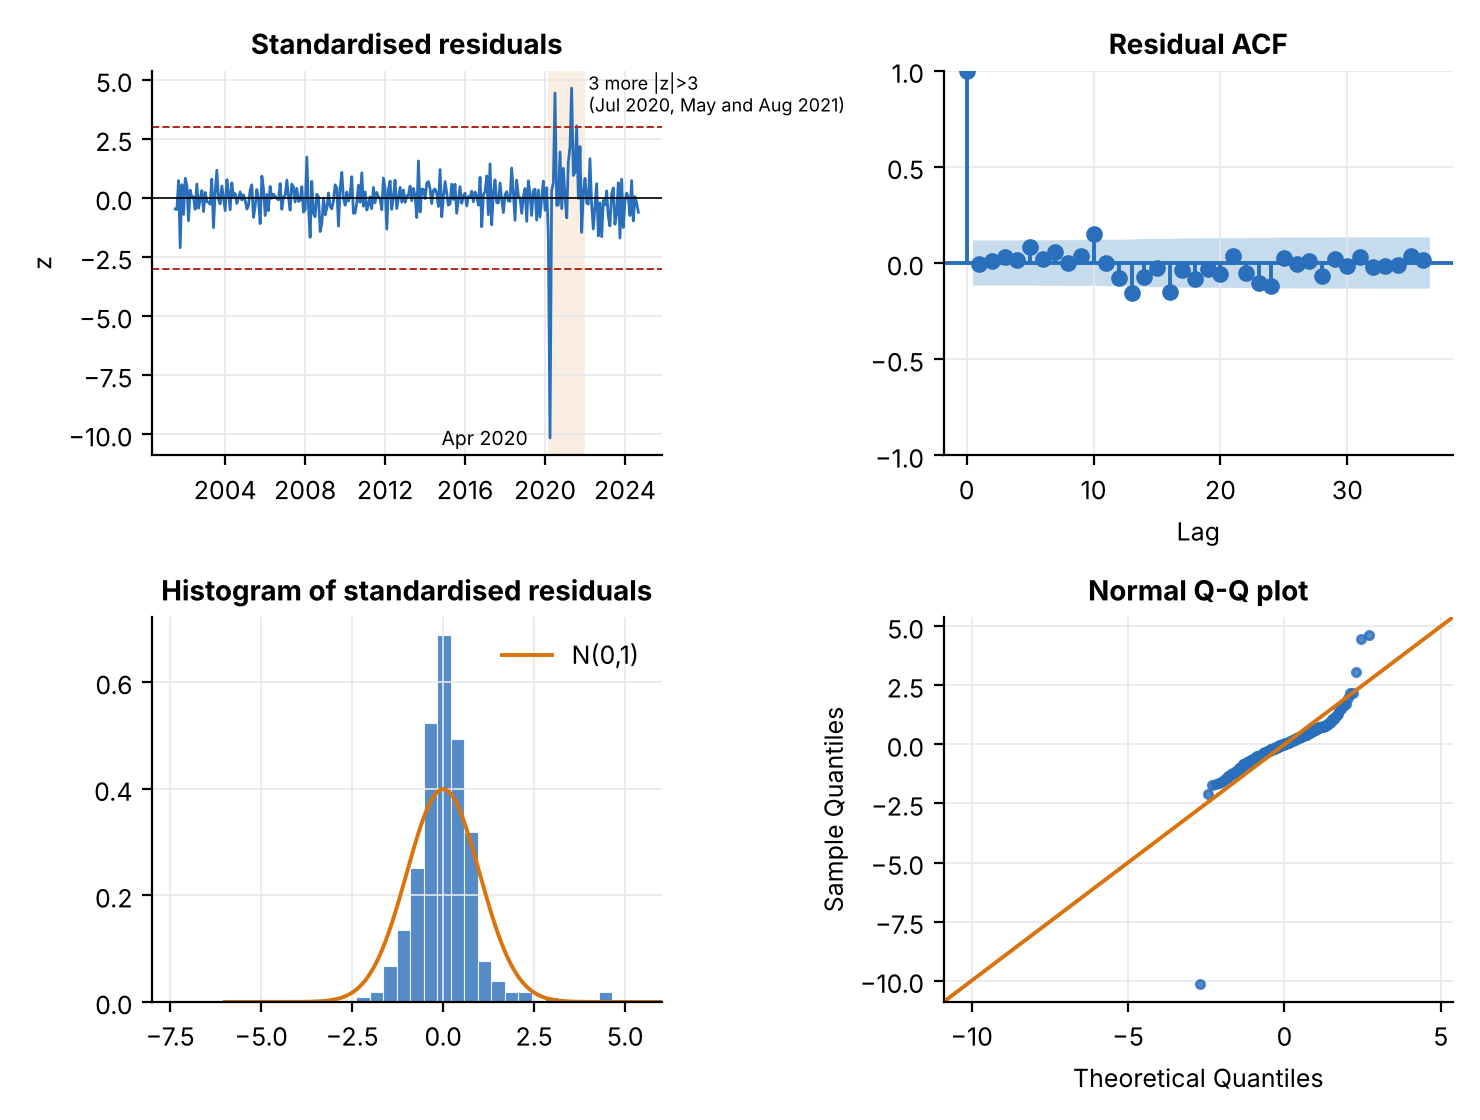
\includegraphics[width=0.97\textwidth]{figures/fig5_residuals.png}
\caption{Diagnostics for $\ARIMA{1}{1}{2}$: standardised residuals through time (dashed lines at $\pm3$; the shaded band is March 2020 -- December 2021); residual ACF with 95\% bands; histogram compared with the standard normal; normal Q--Q plot.}\label{fig:resid}
\end{figure}
\begin{itemize}
\item \textbf{Through time:} residuals look like noise around zero before 2020 and after 2022. In the COVID window there are large spikes: April 2020 is a $-10.2$ standard-deviation event, and July 2020, May 2021 and August 2021 exceed $+3$ ($4.4$, $4.6$, $3.1$). These are genuine shocks that no stationary ARIMA could have anticipated.
\item \textbf{Residual ACF:} almost all bars lie within the band. The first 9 lags are clean (the largest in absolute value is $0.08$). Four bars are outside the 95\% band: lag 10 ($+0.15$), lag 13 ($-0.16$), lag 16 ($-0.15$) and lag 24 ($-0.12$). With 36 lags examined, about two exceedances would be expected by chance at the 5\% level, so four slightly-above-chance exceedances of small size (every $|\hat\rho|\le 0.16$) are a mild finding, not an alarming one. Lag 12 is not significant and lag 24 only just exceeds the band ($-0.118$ vs.\ $0.117$), so there is no clear seasonal pattern, consistent with the ONS statement.
\item \textbf{Histogram and Q--Q:} the bulk of the distribution is close to normal but with a very heavy left tail from April 2020. This is a single-observation feature, as the next subsection shows.
\end{itemize}

\subsection{Formal tests}
\begin{table}[H]\centering\small
\caption{Residual diagnostics for ARIMA(1,1,2) (279 residuals; the first, a diffuse start-up value, is dropped).}\label{tab:diag}
\begin{tabular}{lrr}\toprule Test & Statistic & p-value\\\midrule
Ljung--Box, 6 lags (df $=6-3$) & 2.51 & 0.474\\
Ljung--Box, 12 lags (df $=12-3$) & 12.26 & 0.199\\
Ljung--Box, 18 lags (df $=18-3$) & 30.39 & \textbf{0.011}\\
Ljung--Box, 24 lags (df $=24-3$) & 40.51 & \textbf{0.006}\\
Ljung--Box, 36 lags (df $=36-3$) & 43.32 & 0.108\\
Ljung--Box on squared residuals, 12 lags & 10.95 & 0.534\\
Engle ARCH-LM, 6 lags & 9.76 & 0.135\\
Jarque--Bera, all residuals & 18814.0 & \textbf{0.000}\\
Jarque--Bera, excluding Mar 2020--Dec 2021 & 6.5 & \textbf{0.039}\\
\bottomrule\end{tabular}
\end{table}

\textbf{Ljung--Box.} The statistic $Q(m)=n(n+2)\sum_{j=1}^m \hat\rho_j^2/(n-j)$ tests the null that the first $m$ residual autocorrelations are jointly zero; under the null it is $\chi^2$ with $m-p-q$ degrees of freedom. Results:
\begin{itemize}
\item Lags 6 and 12: no evidence of residual autocorrelation ($p=0.47$ and $0.20$). This is the range that matters for 1-, 3- and 6-month forecasts, and it is also the range in which models with fewer terms clearly fail, e.g.\ $(0,1,2)$ has $p=0.005$ at lag 6.
\item Lags 18 and 24: rejection at 5\% ($p=0.011$ and $0.006$). Figure~\ref{fig:lb} shows the p-value as a function of the number of lags: it is high up to $m\approx 12$, is mostly below 0.05 for $m$ between about 13 and 30 because of the small spikes at lags 10, 13, 16 and 24, and recovers to $p=0.11$ at $m=36$.
\item Competing models do no better: $(1,1,3)$ and $(1,1,4)$ show the same pattern and $(0,1,2)$ fails at every lag (Figure~\ref{fig:lb}). Fitted to the pre-COVID sample only, $(1,1,2)$ fails even at lag 12 ($p<0.001$; lag 24: $p=0.006$), so this feature is in the data, not just a COVID artefact. It is not removed by dummies for the four COVID outliers either (LB(24) $p=0.009$ with dummies).
\end{itemize}
\begin{figure}[H]\centering
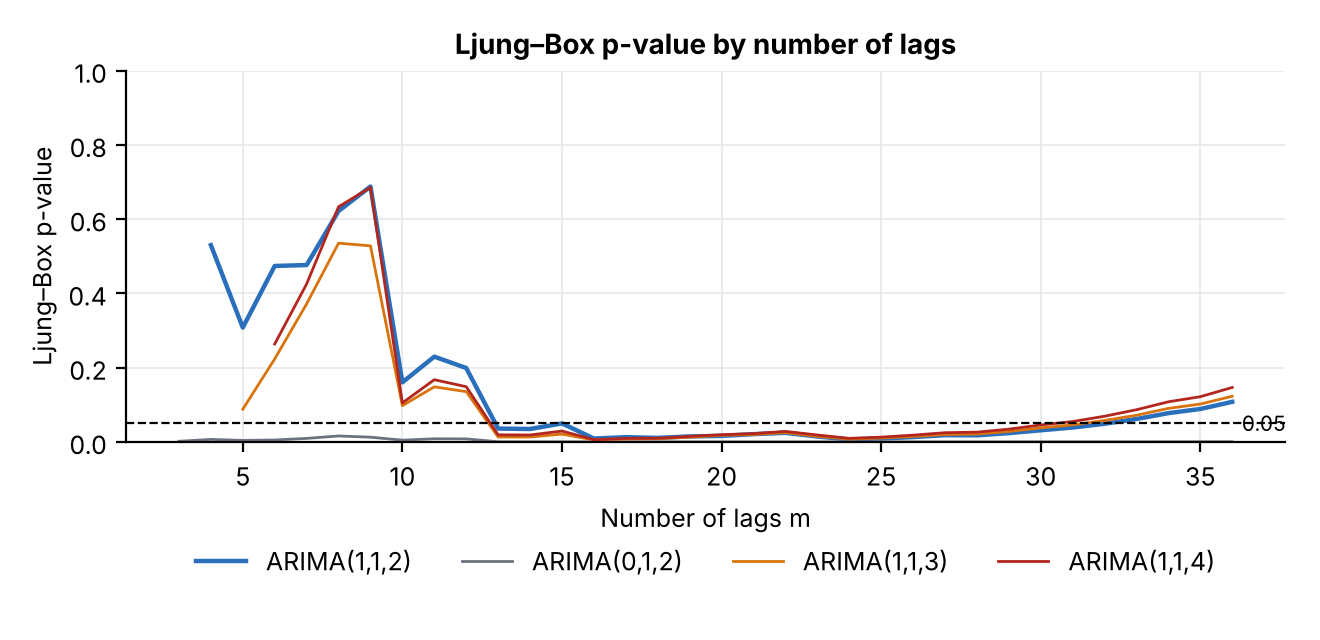
\includegraphics[width=0.78\textwidth]{figures/fig6_ljungbox.png}
\caption{Ljung--Box p-value against the number of lags $m$ for four candidates. All pass at short lags and dip below 0.05 for $m$ from about 13 to 30; $(0,1,2)$ fails at every lag.}\label{fig:lb}
\end{figure}

\textbf{Heteroskedasticity.} The residual standard deviation depends heavily on the period:
\begin{center}\small
\begin{tabular}{lrrr}\toprule
Period & Before Mar 2020 & Mar 2020 -- Dec 2021 & From Jan 2022\\\midrule
Observations & 224 & 22 & 33\\
Residual s.d.\ (thousands) & 7.8 & 38.7 & 10.8\\\bottomrule
\end{tabular}
\end{center}
During the COVID window the residual s.d.\ is nearly five times its pre-2020 value. Even so, the standard ARCH tests do not flag it: Engle's ARCH-LM test with 6 lags gives $p=0.135$ and the Ljung--Box test on squared residuals ($12$ lags) $p=0.53$. I would not read that as clean. ARCH tests look for volatility that clusters and persists, whereas here the volatility is concentrated in one regime of 22 months dominated by a single extreme observation, which is a different (and for these tests less detectable) pattern. The regime table is the more informative evidence. The post-2022 s.d.\ (10.8) is also higher than the pre-2020 value (7.8), partly because the level of vacancies is now higher and the changes larger.

\textbf{Normality.} Over all residuals, normality is strongly rejected (Jarque--Bera $=18{,}814$; skewness $-3.02$; excess kurtosis $39.8$), but this is driven almost entirely by April 2020. Excluding March 2020 -- December 2021, the residuals are close to normal (skewness $-0.28$, excess kurtosis $0.55$; Jarque--Bera $6.5$, $p=0.039$, still a marginal rejection). The Durbin--Watson statistic is $2.00$, a further sign of no first-order autocorrelation.

\subsection{Is the specification appropriate for our research?}
\key{\textbf{Verdict: adequate as a working specification, with three caveats.}\\[2pt]
\textbf{What is good:} the mean structure is captured. Ljung--Box does not reject at lags 6 and 12, the models with fewer terms are clearly worse, and the parameter values have a sensible interpretation.\\[2pt]
\textbf{Caveats:} (i) small residual autocorrelations at lags 10, 13, 16 and 24 (all $|\hat\rho|\le0.16$), which make the Ljung--Box test reject at lags 18--24 and which no candidate model removes; (ii) variance that is about five times larger during the COVID window, so the constant-variance assumption fails; (iii) non-normal residuals driven by April 2020. }

How much this matters depends on how the model is used. For \emph{point forecasts} at horizons of 1--6 months, the small long-lag correlations are unlikely to matter much, because the model's information is in the first few lags. For \emph{prediction intervals}, however, the estimated innovation s.d.\ of $13.3$ is a blend of a quiet regime ($\approx 8$) and the COVID regime ($\approx 39$): Gaussian intervals built on it would be too wide in calm periods and too narrow in a crisis. For the ARIMAX stage, the unmodelled COVID shock could also be wrongly attributed to the Indeed index.

%--------------------------------------------------------------------
\section{Conclusions and suggested next steps}
%--------------------------------------------------------------------
\begin{enumerate}
\item \textbf{Differencing:} $d=1$. The level is non-stationary and the first difference is stationary (ADF and KPSS agree); no second difference is warranted.
\item \textbf{Specification:} $\ARIMA{1}{1}{2}$ without drift, on the level of vacancies. It is first on AIC, AICc and BIC among 50 candidates, and the MA(2) component is a direct and expected consequence of the series being a 3-month rolling average. $\ARIMA{0}{1}{3}$ is a statistical near-tie and is the natural alternative to carry into Week 3.
\item \textbf{Diagnostics:} Ljung--Box does not reject up to lag 12 (one isolated spike at lag 10); mild autocorrelation at lags 10--24 not removed by any candidate; strongly heteroskedastic residuals during COVID; heavy left tail from April 2020.
\end{enumerate}

\textbf{Suggested next steps for the forecasting stage} (these are suggestions for discussion, not things I have done):
\begin{itemize}
\item Report forecast accuracy for $\ARIMA{1}{1}{2}$ and $\ARIMA{0}{1}{3}$ against the naive random walk on the held-out 24 months, re-estimating at each origin, and report the COVID treatment explicitly (full sample versus pre-COVID versus outlier dummies).
\item Use empirical or regime-aware prediction intervals, since the residual variance is not constant.
\item Allow for the overlap in the rolling average when setting the first forecast origins in the hold-out sample (see Section~1.2).
\item Re-run the specification search on the pre-COVID sample alongside the full sample: it favours a longer MA structure $(1,1,4)$ and is a useful check of stability.
\end{itemize}

\textbf{Limitations.} (a) The search over 50 models and the use of the same data for selection and diagnostics means that reported p-values are conditional on selection and are optimistic. (b) The COVID treatment uses dummies chosen after looking at the residuals. (c) The rolling-average structure means observations are not independent monthly measurements; the model describes the \emph{published smoothed series}, not the underlying monthly vacancy count. (d) Near-non-invertibility of the MA(2) part means parameter standard errors are approximate. (e) I did not model the job-openings-rate sheet or any other industry series.

%--------------------------------------------------------------------
\appendix
\section{Top 15 models by BIC}\label{app:top15}
\begin{longtable}{lcrrrrrr}\caption{Top 15 of the 50 grid models ranked by BIC.}\label{tab:top15}\\\toprule
Model & $k$ & AIC & AICc & BIC & LB(12) & LB(24) & Converged\\\midrule\endfirsthead
ARIMA(1,1,2) & 4 & 2247.4 & 2247.5 & 2261.9 & 0.199 & \textbf{0.006} & yes\\
ARIMA(0,1,3) & 4 & 2248.0 & 2248.2 & 2262.6 & 0.151 & \textbf{0.003} & yes\\
ARIMA(0,1,2) & 3 & 2254.8 & 2254.9 & 2265.7 & \textbf{0.008} & \textbf{0.000} & yes\\
ARIMA(1,1,3) & 5 & 2249.0 & 2249.2 & 2267.2 & 0.135 & \textbf{0.007} & yes\\
ARIMA(2,1,2) & 5 & 2249.2 & 2249.5 & 2267.4 & 0.151 & \textbf{0.005} & yes\\
ARIMA(1,1,2)$+$drift & 5 & 2249.3 & 2249.6 & 2267.5 & 0.199 & \textbf{0.006} & yes\\
ARIMA(0,1,4) & 5 & 2249.6 & 2249.8 & 2267.7 & 0.129 & \textbf{0.003} & yes\\
ARIMA(0,1,3)$+$drift & 5 & 2250.0 & 2250.2 & 2268.2 & 0.151 & \textbf{0.003} & yes\\
ARIMA(0,1,2)$+$drift & 4 & 2256.8 & 2256.9 & 2271.3 & \textbf{0.008} & \textbf{0.000} & yes\\
ARIMA(1,1,4) & 6 & 2249.6 & 2249.9 & 2271.4 & 0.148 & \textbf{0.009} & yes\\
ARIMA(2,1,3) & 6 & 2249.8 & 2250.1 & 2271.6 & 0.142 & \textbf{0.009} & yes\\
ARIMA(3,1,2) & 6 & 2250.8 & 2251.1 & 2272.5 & 0.118 & \textbf{0.005} & yes\\
ARIMA(1,1,3)$+$drift & 6 & 2251.0 & 2251.3 & 2272.8 & 0.136 & \textbf{0.007} & yes\\
ARIMA(2,1,2)$+$drift & 6 & 2251.2 & 2251.5 & 2273.0 & 0.151 & \textbf{0.005} & yes\\
ARIMA(0,1,4)$+$drift & 6 & 2251.5 & 2251.9 & 2273.3 & 0.129 & \textbf{0.003} & yes\\
\bottomrule\end{longtable}

\section{Files delivered}
\sloppy
\begin{itemize}
\item \texttt{analysis.py}: full script (tests, 50-model grid, diagnostics, robustness, figures, tables).
\item \texttt{tables/arima\_grid\_full.csv}: all 50 fitted models (AIC, AICc, BIC, $\Delta$IC, Ljung--Box p-values, convergence); \texttt{tables/shortlist.csv}: the comparison table of Table~\ref{tab:candidates}; \texttt{tables/stationarity\_tests.csv}: every ADF and KPSS result; \texttt{tables/robustness.csv}; \texttt{tables/levels\_vs\_log.csv}; \texttt{tables/recommended\_residuals.csv}.
\item \texttt{figures/}: the seven figures used above.
\end{itemize}
\end{document}
